\subsection{Workflow Mechanismus}

Kobold bietet dem Benutzer einen Workflow-Mechanismus, der ihn bei
der Einhaltung des definierten produktlinienbasierten
Entwicklungsprozesses unterst�tzt. Dieser f�hrt
Konsistenzpr�fungen durch, die in anderen Client-Instanzen
automatisch Workflows ansto�en, um erkannte Inkonsistenz zu
beheben. Zur Realisierung des Workflow-Mechanismus wird die 'Rule
Engine' Drools\footnote{http://www.drools.org} verwendet, welche
eine funktional orientierte, intelligente Wissensbasis modelliert,
die auf Fakten Antworten generiert (�hnlich den PROLOG Prinzipien
aus der Logik-Vorlesung).\par Daf�r wird eine Regelbasis in XML
f�r Drools erzeugt. Diese besteht aus einer Menge von Regelmengen
und wird vom Serverdienst persistiert. Eine Regelmenge
besteht aus einzelnen Regeln, durch die verschiedene
Pr�fungen vorgenommen werden k�nnen.\par Eine solche Regel
besteht aus drei Teilen:
\begin{itemize}
\item Parameter
\item Bedingung
\item Konsequenz
\end{itemize}
\paragraph{Parameter} sind Eingaben (Fakten), die auf die
jeweiligen Regeln angewendet werden.
\paragraph{Bedingungen} entscheiden anhand der Parameter, welche
Konsequenzen ausgef�hrt werden.
\paragraph{Konsequenzen} dienen zur Erzeugung/Modifikation von
Workflow-Objekten, falls eine Bedingung zutrifft.\par
Fakten werden auf alle Regeln einer Regelmenge angewendet.\par
Der Workflow-Mechanismus ist eine Querschnittskomponente zwischen dem
Kobold Serverdienst und dem Kobold-Client.

\subsubsection{Mechanismus auf dem Kobold Client}
Der Kobold Client ruft zu bestimmten Zeitintervallen (Standard:
im Minutentakt) Nachrichten vom Server ab. Nachrichten k�nnen
RPC-Resultate sein, aber auch Workflow-Objekte. Wird ein
Workflow-Objekt abgerufen, so erscheint dieses Objekt in der
Workflow/Task View und kann per Doppelklick detailliert betrachtet
werden.\par 
Der Workflow-Mechanismus kann
wie folgt graphisch veranschaulicht werden:
\begin{figure}[h!]
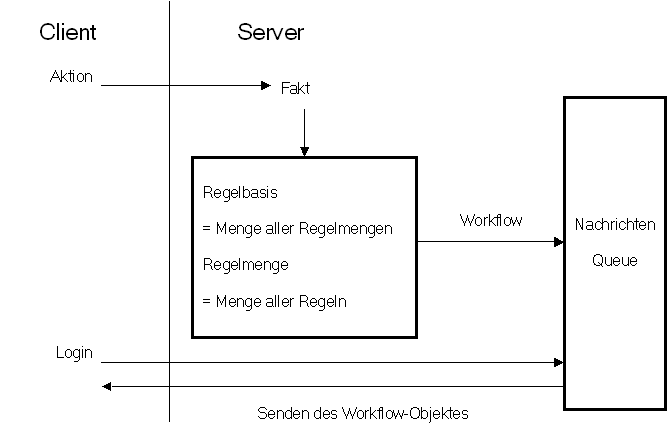
\includegraphics[width=15cm]{drools.png}
   \caption{Workflow Mechanismus}
\end{figure}

\subsubsection{Die Regelbasis in Kobold}
Kobold wird nach der ersten Iteration eine Initialregelbasis zur
Verf�gung stellen, die vom Anwender jederzeit erweitert werden
kann. Er muss dabei eine neue Regel erstellen und sie der
Regelbasis hinzuf�gen. Die Konsequenzen solcher Regeln m�ssen
nicht notwendigerweise Workflow-Objekte erzeugen, sondern k�nnen
auch andere Aktionen ausf�hren. Der
Mechanismus ist sehr flexibel erweiterbar. \par Zur Erstellung
einer neuen Regel kann der Workflow-Editor verwendet werden, der
in einer sp�teren Iterationen realisiert wird.
